\documentclass[12pt]{report}
\usepackage[T1]{fontenc}
\usepackage[utf8]{inputenc}
\usepackage[spanish]{babel}
\usepackage{amsmath, amsthm, amssymb, graphicx, subcaption, enumerate, hyperref, tikz, pgfplots, verbatim, pdfpages}
\usepackage[algochapter]{algorithm2e}
\usetikzlibrary{matrix}
%\usepackage[]{algorithm2e}
%\usepackage[top=1.5in, bottom=1.5in, left=1.5in, right=1.5in]{geometry}
%\usepackage{geometry}
 
%\addtolength{\oddsidemargin}{-.875in}
%\addtolength{\evensidemargin}{-.875in}
%\addtolength{\textwidth}{1.75in}
%\addtolength{\topmargin}{-.875in}
%\addtolength{\textheight}{1.75in}
\addtolength{\footskip}{5pt} % Para que los numeros no esten tan pegados al texto

%\renewcommand\figurename{Figura}
\renewcommand\spanishtablename{Tabla}
% NOTAR QUE HAY QUE PONERLE SPANISH LALA AL USAR BABEL
%\renewcommand\spanishcontentsname{\'Indice general}
\renewcommand\spanishlistfigurename{\'Indice de figuras}
\renewcommand\spanishlisttablename{\'Indice de tablas}
%\renewcommand\spanishchaptername{Cap\'itulo}
%\renewcommand\bibname{Bibliograf\'ia}
\SetAlgorithmName{Algoritmo}{algoritmo}{Lista de Algoritmos}


\newcommand{\R}{\mathbb{R}}
\newcommand{\signo}{\text{ signo}}
\newcommand\eq{=}
\newcommand{\minimizar}[1]{\underset{#1}{\text{minimizar}} \;}

\newtheorem{teo}{Teorema}[chapter]
\newtheorem{defn}{Definici\'on}[chapter]
\newtheorem{regla}{R}%[chapter]
\newtheorem{prop}{Proposici\'on}[chapter]
\newtheorem{cor}{Corolario}[chapter]
\newtheorem{lema}{Lema}[chapter]
\newtheorem{obs}{Observaci\'on}[chapter]
 
 %%%%%%%%%%%%%%%%%%%%%%%%%%%%%%%%%%%%%%%%%%%%%%%%%%%%
\begin{document}

%%%%%%%%%%%%%%%%%%%%%%%%%%%%%%%%%%%%%%%%%%%%%%%%%%%%
% PORTADA 1a HOJA IMPRESA
%\includepdf{CaratulaTesisFelipe.pdf}
\pagenumbering{gobble}
{\large
\begin{center}
INSTITUTO TECNOL\'OGICO AUT\'ONOMO DE M\'EXICO
\end{center}
\begin{figure}[h]
 	\centering
	
\includegraphics[width=0.4\textwidth]{imagenes/logo_ITAM.jpg}
	\end{figure}
\begin{center}
\vspace{0cm}
\textbf{SISTEMA DE RECOMENDACIÓN DE HOTELES SIMILARES}\\
\vspace{1cm}
TESIS\\
\vspace{1cm}
{\normalsize QUE PARA OBTENER EL T\'ITULO DE}\\
\vspace{0.5cm}
MAESTRO EN CIENCIA DE DATOS\\
\vspace{0.5cm}
{\normalsize PRESENTA}\\
\vspace{1cm}
FELIPE GERARD VALD\'ES\\
\vspace{2cm}
{\normalsize ASESOR: [Si me dejan] NADIA DEL VILLAR}\\
\vspace{2cm}
\end{center}
\begin{flushleft}
M\'EXICO, D.F.\hfill 2015%\phantom{20144}
\end{flushleft}
}
 
%%%%%%%%%%%%%%%%%%%%%%%%%%%%%%%%%%%%%%%%%%%%%%%%%%%% 
% DISCLAIMER
\newpage
\noindent``Con fundamento en el art\'iculo 21 y 27 de la Ley Federal del Derecho de Autor y como titular de los derechos moral y patrimonial de la obra titulada \textbf{``SISTEMA DE RECOMENDACIÓN DE HOTELES SIMILARES'}, otorgo de manera gratuita y permanente al Instituto Tecnológico Aut\'onomo de M\'exico y a la Biblioteca Ra\'ul Bailleres Jr., autorizaci\'on para que fijen la obra en cualquier medio, incluido el electr\'onico, y la divulguen entre sus usuarios, profesores, estudiantes o terceras personas, sin que pueda percibir por tal divulgaci\'on una contraprestaci\'on"
\vspace{40pt}
\begin{center}
\textbf{Felipe Gerard Vald\'es}\vspace{2cm}\\
\noindent\begin{tabular}{c}
\makebox[2in]{\hrulefill}\\
FECHA\vspace{2cm}\\
\makebox[2in]{\hrulefill}\\
FIRMA
\end{tabular}
\end{center}

\pagenumbering{Roman} % para comenzar la numeracion de paginas en numeros romanos



% ----------------------------------------------------------------------------------------------------
\tableofcontents
\listoffigures
\listoftables
 
% ----------------------------------------------------------------------------------------------------
\addcontentsline{toc}{chapter}{Pr\'ologo}
\chapter*{Pr\'ologo}
\pagenumbering{arabic}

% ----------------------------------------------------------------------------------------------------
\chapter{Análisis previo}

Antes de desarrollar el modelo de recomendación de hoteles similares, es conveniente analizar el \emph{status quo}. Comenzaremos con un análisis de la competencia del que trataremos de sacar información valiosa de qué hay o no hay en el mercado y tomar ideas, posteriormente haremos un análisis del sistema de Best Day que pretendemos mejorar con el fin de entender en dónde hay áreas de oportunidad y finalmente sacaremos conclusiones de lo aprendido.

\section{Sistemas actuales}

En esta sección analizaremos la manera en que la competencia de Best Day recomienda hoteles y luego veremos qué se hace en Best Day. Los ámbitos que nos interesan son
\begin{enumerate}
	\item La posición dentro de la página de las recomendaciones.
	\item La forma en la que se eligen las recomendaciones.
\end{enumerate}
Enfatizaremos en los principales competidores, de Best Day, es decir: Booking, Price Travel, Expedia y Despegar. También veremos si podemos aprender algo de TripAdvisor, que aunque no es un competidor directo, vive de recomendar hoteles y de su comunidad de comentarios. Las empresas competidoras están ordenadas de menor a mayor relevancia del sistema de recomendación que tienen.

\subsection*{Price Travel (pricetravel.com)}

Pusimos a Price Travel en primer lugar en la lista porque no tienen un sistema de recomendación de hoteles similares. Cuando se busca un destino, se presentan los hoteles en el Sort Order determinado por su sistema, pero ya que se entra a la página de un hotel en particular (independientemente de cómo se llegó a esa página), no se recomienda hoteles similares ni cercanos. De hecho, la única indicación de otros hoteles es en la pestaña de mapa, en la que se pueden ver todos los cercanos en un mapa interactivo. Dado que no aprendimos nada de este competidor, procederemos al siguiente.

\subsection*{Booking (booking.com)}

Booking es un competidor muy importante de Best Day, aunque también tiene un mercado más granda y mayor cantidad de opciones en destinos fuera de Latinoamérica. Antes de entrar en los puntos de interés general, cabe mencionar que algo que hace booking que no hacen los demás es que cuando se busca un hotel en la página con la barra inteligente, en lugar de ir directamente a su página, se muestra en el primer lugar de una lista, dando la posibilidad de elegir algún otro hotel. Ahora sí pasemos al tema en cuestión:
\begin{itemize}
	\item \textbf{Hoteles populares por destino}
	\begin{enumerate}
		\item Se encuentran del lado izquierdo, abajo de la barra de búsqueda y fechas. Es una posición de prominencia media-baja, puesto que no es visible inmediatamente sin bajar en la página.
		\item Cuando se entra a la página (no al hotel en particular) por primera vez y se selecciona un hotel, aparece una sección de hoteles populares en el mismo destino del hotel buscado. El tema es que siempre aparece la misma selección para cada destino, independientemente del hotel que se haya elegido, pues la popularidad de los otros hoteles no tiene relación con el hotel elegido.
	\end{enumerate}
	\item \textbf{Búsquedas recientes}
	\begin{enumerate}
		\item Se encuentran en el mismo lugar que los hoteles populares por destino, pero los sustituyen una vez que se ha visitado al menos un hotel anteriormente.
		\item La información de los hoteles visitados se va almacenando en una \emph{cookie}, de modo que para los hoteles subsecuentes, en lugar de los hoteles populares por destino, aparece un listado de unos pocos hoteles recientemente buscados por el usuario.
	\end{enumerate}
\end{itemize}
Al parecer en Booking sólo están interesados en lo que el cliente ha buscado y utilizan los hoteles populares por destino para no dejar vacía la sección para los clientes nuevos. El problema con los hoteles populares por destino es que no varían según el hotel buscado (siempre y cuando estén en el mismo destino), mientras que el de las búsquedas recientes es que no promueven que el cliente explore la página y encuentre la mejor opción para sus necesidades. Entraremos en detalles más adelante.

\subsection*{Despegar (despegar.com)}

Despegar es un competidor más directo y con un mercado más parecido al de Best Day que Booking, aunque está más enfocado en vender boletos de avión que cuartos de hotel. En este caso hay más de una estrategia y en más de un lugar de la página de cada hotel, por lo que las describiremos por separado. Cabe mencionar que no usan todas las estrategias para todos los hoteles, por lo que sospechamos que tienen información incompleta y sólo muestran lo que tienen disponible.
\begin{itemize}
	\item \textbf{Búsquedas recientes}
	\begin{enumerate}
		\item Se encuentra en la izquierda abajo del mapa. Igual que en booking.com, se tiene que bajar en la página para verlo, por lo que su relevancia es media-baja.
		\item Son los hoteles buscados recientemente por el usuario. Curiosamente, no siempre nos aparecieron al hacer búsquedas, incluso después de haber visto varios hoteles.
	\end{enumerate}
	\item \textbf{Hoteles cercanos}
	\begin{enumerate}
		\item Se encuentra directamente debajo de las búsquedas recientes.
		\item Se listan los hoteles más cercanos al hotel en buscado, sin ningún criterio de precio, categoría o estilo del hotel.
	\end{enumerate}
		\item \textbf{Hoteles populares por destino}
	\begin{enumerate}
		\item Se encuentra directamente abajo de los hoteles cercanos.
		\item Para cada destino muestra una lista de los hoteles más populares (presumiblemente los más vendidos). La lista es la misma para todos los hoteles en un destino dado y de hecho contiene al hotel buscado en su posición correspondiente (es decir ni se omite ni aparece hasta arriba).
	\end{enumerate}
	\item \textbf{Otros usuarios también buscaron...}
	\begin{enumerate}
		\item Aparece en la parte inferior de la página, abajo de prácticamente todo. Su relevancia es muy baja y de hecho se omitió en los primeros análisis de la competencia porque no lo vimos.
		\item En la parte inferior de la página también aparece una sección de hoteles que fueron visitados por los demás usuarios que han visto el hotel en cuestión. Este análisis no es complejo, pero puede ser pesado computacionalmente si no se utilizan métodos apropiados de \emph{Market Basket Analysis} como el algoritmo \emph{A Priori}, por ejemplo.
	\end{enumerate}
\end{itemize}
En Despegar tuvieron muchas ideas para recomendar, pero todos los criterios están separados y no colaboran entre sí. Es como tener una tabla ordenada por varios campos distintos. Los hoteles recomendados con base en lo que han visto otros clientes creemos que están desperdiciados en donde están, puesto que sólo los clientes que vayan hasta abajo de la página los verán. El sistema funciona razonablemente bien y permite movilidad hacia arriba en la categoría del hotel. El problema es que es claramente afectado por la popularidad de los hoteles, de modo que tiende a atorarse en aglomerados de hoteles populares y también a subir de categoría. El resultado es que después de algunos pocos \emph{clicks}, casi invariablemente se llega a los hoteles más caros de la zona, sin posibilidad de explorar otros.

\subsection*{Expedia (expedia.com)}

En Expedia se le da una prioridad bajísima a las recomendaciones, puesto que están posicionadas en un lugar casi imposible de ver. Sin embargo, tienen un sistema diferente a los demás y por eso lo pusimos en esta posición en la lista de sistemas competidores.
\begin{itemize}
	\item \textbf{Búsquedas recientes}
	\begin{enumerate}
		\item Se encuentran en el centro, casi hasta abajo, después de toda la información del hotel. La prioridad es muy baja.
		\item Es igual que en las demás páginas. Aparecen los últimos cuatro hoteles buscados distintos del actual (en caso de repetir una búsqueda).
	\end{enumerate}
	\item \textbf{Hoteles recomendados}
	\begin{enumerate}
		\item Se encuentran directamente abajo de las búsquedas recientes.
		\item Utilizan un método desconocido para recomendar hoteles similares que permite movilidad progresiva entre categorías. No estamos seguros si tiene alguna restricción de precios.
	\end{enumerate}
\end{itemize}
El sistema de recomendación de Expedia nos gustó bastante y de hecho creemos que lo están desaprovechando. Permite explorar los hoteles disponibles con hacia arriba y hacia abajo en la escala de precio y categoría y llegar a opciones completamente nuevas. Es probable que esté acotado por destino, aunque eso no es tan grave. Algo que no nos gustó tanto es que tal vez es algo rígido y después de buscar un poco se puede atorar. A diferencia del algoritmo de Booking, esto no necesariamente lleva a los hoteles más caros de la zona.

\subsection*{Trip Advisor (tripadvisor.com)}

Como decíamos arriba, Trip Advisor no es la competencia directa de Best Day, pero es un sitio muy popular de evaluación de hoteles y creemos que podemos aprender de ellos.
\begin{itemize}
	\item \textbf{Hoteles similares}
	\begin{enumerate}
		\item Se encuentran en la derecha, abajo de la foto principal, pero al lado de otra información importante, por lo que el impacto es medio.
		\item No sabemos cómo hacen las recomendaciones, pero no son por distancia estricta y sí permiten cierta movilidad de la categoría.
	\end{enumerate}
\end{itemize}
El sistema de TripAdvisor también funciona razonablemente bien, pero parece estar más basado en la calificación de los usuarios que en la categoría del hotel. Si bien ese enfoque tiene sentido en el contexto de su página, Best Day no tiene información tan detallada como ellos en cuanto a lo que opinan los usuarios y además el enfoque es distinto. Algo que tampoco nos gustó es que el sistema es bastante rígido y se puede quedar atorado fácilmente en ciertos grupos de hoteles.

\subsection*{Best Day (bestday.com.mx)}

Finalmente, analizaremos lo que se hace actualmente en Best Day. Del mismo modo que con la competencia, comenzaremos con una breve descripción:
\begin{itemize}
	\item \textbf{Hoteles similares}
	\begin{enumerate}
		\item Los hoteles similares están abajo de la liga al mapa del lado derecho. Como en la mayoría de los competidores, no se ve inmediatamente al entrar en la página, por lo que tiene prominencia media-baja.
		\item La manera de recomendar hoteles es por categoría (estrellas) y por destino, es decir, se toman los hoteles de las mismas estrellas y en el mismo destino que el hotel buscado y se presentan en el Sort Order del momento. No se toma en cuenta el precio ni la distancia (salvo por el hecho de encontrarse en el mismo destino) de las opciones.
	\end{enumerate}
	\item \textbf{Búsquedas recientes}
	\begin{enumerate}
		\item Se encuentran directamente debajo de los hoteles similares.
		\item Similarmente a la competencia, aparece una lista de los hoteles que el usuario visitó recientemente. Las búsquedas recientes permanecen entre sesiones dentro de una misma computadora.
	\end{enumerate}
\end{itemize}
Al parecer las búsquedas recientes son (casi) un estándar en la industria, por lo que es confortante saber que Best Day es competitiva en este ámbito. Por otro lado, la calidad de las recomendaciones es muy variable. En zonas homogéneas y con mucha oferta para una categoría dada, las recomendaciones pueden ser razonablemente buenas. Sin embargo, en destinos donde hay hoteles muy distintos pero con la misma categoría, como podrían ser un hotel citadino y uno de playa, las recomendaciones dejan mucho que desear. Además, si no hay o casi no hay hoteles bajo este criterio, no se muestra nada, o casi nada. Más adelante expondremos estos temas con más detalle.

\section{Diagnóstico}

Antes de describir lo que nos gustaría que hiciera el algoritmo de recomendación, resumiremos lo que aprendimos de analizar las diversas páginas. En primer lugar, nos dimos cuenta de que poner una sección con las búsquedas recientes es algo muy deseable y relativamente fácil de implementar. De hecho, es un estándar en la industria, pues todos los competidores lo tienen, a excepción de Price Travel. Sin embargo, recomendar hoteles que el cliente ya vio no cuenta realmente como recomendaciones y debería manejarse en un plano separado. Posiblemente se podría utilizar información de los hoteles visitados en las recomendaciones, pero por ahora proponemos dejar intacta esta sección.

Quitando las búsquedas recientes de en medio, podemos analizar los diversos sistemas de recomendación. Un punto que pensamos que es sumamente importante es el precio. Hasta donde pudimos ver, ninguna página tiene miramiento alguno con el costo de los hoteles recomendados. El resultado es que pueden recomendar hoteles del doble o incluso triple de precio que el original. Creemos que esto no promueve que el cliente explore más alternativas, ya que la mayoría basa su decisión fuertemente en el precio de los hoteles. Propondremos una forma simple de lidiar con este problema sin perder flexibilidad en las recomendaciones.

Otro factor que nos pareció mejorable es el uso de la información geográfica. Parece ser que la opción más popular es únicamente utilizar la información incluida en el destino y, de hecho, parece que sólo Despegar tiene una sección de hoteles más cercanos. Si bien utilizar el destino como punto de partida es una opción razonable, creemos que se podría aprovechar mejor la información si se utilizan las coordenadas geográficas, dado que en la vida real lo que realmente importa es la proximidad de los hoteles; los destinos son particiones más o menos arbitrarias que no deberían afectar las recomendaciones. Por ejemplo, se puede recomendar un hotel en Cancún dado que se buscó un hotel en la zona norte de la Riviera Maya, o uno en Playa del Carmen a una persona que buscó algo en Cozumel. 

Un tercer problema con el que nos encontramos en las recomendaciones es que en la mayoría de los casos eran estáticas. Es decir, son idénticas para ciertos grupos de hoteles. Esto pasa en todas las opciones que vimos que utilizan el destino (Booking, Despegar, Best Day) como criterio, pues no dependen también del hotel. Esto en sí mismo puede ser un problema en destinos amplios, además de que el usuario agota las recomendaciones rápidamente, volviéndolas inútiles. 

En cuarto lugar, nos dimos cuenta que en varias de las páginas se han dado cuenta de que quieren recomendar hoteles vía varios criterios, pero muchas veces no los integran. La estrategia tiende a ser usar un criterio para ordenar a la vez, en lugar de aprovechar varios simultáneamente. Esto contribuye al tercer punto, pues hay poco cambio en las recomendaciones de hotel a hotel.

En quinto lugar, notamos que en general los sistemas que sí recomendaban de forma más sofisticada resultaban rígidos y/o se podían quedar atorados fácilmente en grupos aislados de hoteles. Esto hace que el sistema se vuelva inútil una vez que se llegó a uno de estos grupos absorbentes. El único que nos pareció decente en este sentido es el de Expedia, aunque sí es algo más rígido de lo que nos gustaría. Otro punto sobre los sistemas en general, pero de los de hoteles similares en particular, es que en ninguna página (salvo tal vez Trip Advisor) aparecen en posiciones de importancia alta. En el mejor de los casos aparecen una página abajo de la principal, al lado, y en los peores casos están hasta abajo. Creemos que están desaprovechando mucho el potencial de dichos sistemas.

Finalmente, un problema particular del sistema de Best Day es que no toma en cuenta de ninguna forma el perfil del hotel. Como mencionamos arriba, no es lo mismo un hotel de playa de cuatro estrellas que un hotel de ciudad de cuatro estrellas, y si por alguna razón ambos están en el mismo destino, como puede suceder en ciudades cerca del mar, por ejemplo, el sistema de recomendación por destino y estrellas puede fallar catastróficamente. Tenemos ejemplos de hoteles de negocios en Cancún para los que se recomienda hoteles todo incluido en la zona hotelera. Esto no es viable y claramente es importante que el algoritmo que desarrollemos tome en cuenta el perfil de los hoteles, sobre todo porque busca recomendar hoteles \emph{similares}.

% ----------------------------------------------------------------------------------------------------
\chapter{Sistema de recomendación de hoteles}

En el capítulo anterior analizamos los sistemas de recomendación que tienen actualmente tanto los competidores como Best Day y expusimos los principales puntos débiles que encontramos. Ahora podemos utilizar el conocimiento obtenido para generar un sistema nuevo que tenga un mejor desempeño y propiedades más deseables que los que vimos. Primero describiremos punto por punto qué nos gustaría que hiciera el sistema y posteriormente dedicaremos una sección para profundizar en cómo resolvimos cada uno de los problemas.

\section{Modelo propuesto}

Para resolver los problemas expuestos en el capítulo anterior proponemos las siguientes medidas:
\begin{enumerate}
	\item Poner una cota superior al \textbf{precio} de los hoteles recomendados, como un porcentaje del precio del hotel buscado.
	\item Recomendar hoteles razonablemente \textbf{cercanos} al buscado, donde el criterio de cercanía varía según la densidad de hoteles en la zona.
	\item Las recomendaciones deben tener un \textbf{perfil} o filosofía similar al original.
	\item Las recomendaciones deben ser hoteles no necesariamente de las mismas estrellas, pero sí deben tener una cantidad similar de \textbf{servicios} disponibles.
\end{enumerate}
Antes de entrar a una descripción detallada de cada medida, explicaremos brevemente cómo colaborarán a que nuestro sistema de recomendación tenga las propiedades que buscamos.

Siempre y cuando dos hoteles sean genuinamente similares a los ojos de una persona, la vasta mayoría de los clientes siempre preferirá el más económico. Acotando el precio esperamos que rara vez aparezcan hoteles más allá de las posibilidades del cliente en las recomendaciones. En cuanto a la distancia entre hoteles, creemos que utilizar la distancia al hotel en cuestión es mucho más razonable que usar el mismo criterio del destino para todos, puesto que promoverá hoteles cercanos además de parecidos en otros sentidos.

Esperaríamos que las similitudes de perfil y servicios trabajen conjuntamente con el criterio de cercanía para obligar a que las recomendaciones varíen de hotel a hotel, incluso dentro de un mismo destino. La ventaja de esto es que se puede explorar muchas opciones sin tener que buscar nada explícitamente, puesto que las recomendaciones abren nuevas alternativas por sí solas. Es importante que demos suficiente flexibilidad al método para que no sea rígido y no se estanque en grupos reducidos de hoteles.

Como último punto, no queremos utilizar estos criterios de forma aislada, pues cada uno tiene diversas faltas. Lo que queremos es integrarlos todos en un sistema poderoso que evite que el cliente tenga que pensar demasiado y que genuinamente le proponga alternativas interesantes. Para ello generaremos una medida de similitud entre los hoteles y mostraremos los más parecidos que estén a una distancia y precio razonables del hotel original. En las siguientes secciones describiremos cada uno de los criterios con mayor nivel de detalle.

Para facilitar la exposición le daremos nombres a los hoteles que van superando cada etapa, hasta llegar a las recomendaciones para cada hotel.
\begin{defn}[Conjunto de hoteles]
Denotamos el conjunto de todos los hoteles por $\mathcal{H}$ y al número de hoteles por $N$, es decir $N = \mathcal{H}$.
\end{defn}

\section{Precio}

Dado que el precio es un factor determinante en la elección de un hotel para la mayoría de los clientes, es importante respetar sus posibilidades económicas a la hora de recomendar nuevas opciones. Es razonable pensar que dados dos hoteles idénticos, un cliente siempre elegirá el más barato, salvo tal vez unos pocos clientes de súper lujo. Por esta razón, decidimos no imponer ninguna cota inferior al precio de los hoteles recomendados, siempre y cuando cumplan los criterios de similitud que describiremos más adelante. Por otro lado, como puede ser desalentador que las sugerencias contengan opciones demasiado caras, optamos por poner una cota superior al precio de los hoteles. Como en este paso queremos reflejar los precios ``reales'' de los hoteles, utilizaremos su precio de largo plazo para generar el filtro, como se explica a continuación.
\begin{regla}[Filtro de precio de largo plazo]
Sea $\gamma \geq 0$ y sea
\[
p^D_i = \frac{\text{Importe total del hotel $i$ en el periodo $D$}}{\text{Total de noches del hotel $i$ en el periodo $D$}}
\]
el precio de largo plazo del hotel $i$ en el periodo $D$. Entonces definimos la cota superior de precio para $i$ por 
\[
p^{sup}_i = (1 + \gamma)p^D_i,
\]
es decir, se exluyen del análisis para $i$ todos los hoteles $j$ con $p^D_j > p^{sup}_i$. Los hoteles restantes están contenidos en el conjunto
\[
\mathcal{H}_i^1 = \{j \in \mathcal{H} : p^D_j > p^{sup}_i\}
\]
\end{regla}
El parámetro $\gamma$ es esencialmente el porcentaje por encima del precio de $i$ que se permitirá que tengan las recomendaciones. Por ejemplo, si $\gamma = 0.3$, entonces se ignoran todas las opciones que sean más de 30\% más caras que $i$. El periodo $D$ debe ser suficientemente largo para que refleje los precios promedio de un hotel, pero no tanto como para que se vea demasiado afectado por la inflación y otros factores. Una buena elección es por ejemplo un año o dos años, pues así además se toma en cuenta los cambios de precios en las diversas temporadas del año. Cabe notar que en esta versión del modelo, tanto $\gamma$ como $D$ son los mismos para todo hotel $i$.

En pruebas empíricas nos gustó el desempeño de $\gamma$ alrededor de 0.3, ya que permite suficiente flexibilidad en los precios y las categorías sin proponer opciones excesivamente costosas.

\section{Distancia: filtro estático}

Antes de entrar en criterios dinámicos de distancia y en similitudes de hoteles, es importante pensar si su cálculo es factible. El tema es que si bien en teoría sería suficiente calcular las similitudes de los hoteles y luego quedarnos con los cercanos, en la práctica esto es complicado. Cuando se quiere conocer la distancia entre cualesquiera dos hoteles de entre, supongamos, $N$ opciones, es necesario almacenar $(N^2 - N)/2$ números (una de las porciones triangulares de la matriz de distancias, quitando la diagonal). Para $N$ incluso moderadamente grande, la cantidad de información a guardar se vuelve prohibitiva. Para empeorar las cosas, los criterios de similitud que desarrollaremos más adelante no son simétricos, por lo que tendríamos que almacenar toda la matriz (menos la diagonal), lo que resultaría en $N^2 - N$ números.

El problema con lo anterior es que además la gran mayoría de los cálculos se desperdiciarían, ya que en nuestro contexto no tiene mucha utilidad guardar la similitud entre un hotel en Veracruz y otro en Las Vegas. Una manera de resolver este problema es ignorar hoteles que seguro no recomendaremos. Dado que queremos que el sistema regrese hoteles similares \emph{y} cercanos, es razonable ignorar los que estén más lejos que una cantidad fija suficientemente grande en cualquier destino.

Hay diversas fórmulas para calcular la distancia geodésica entre dos puntos, unas más sofisticadas que otras. Sin embargo, como en este caso estamos interesados en hoteles cercanos, basta con la versión que supone que la Tierra es esférica:
\begin{defn}[Distancia geodésica]
Definimos la distancia geodésica (en kilómetros) entre dos puntos $x = (x_{long}, x_{lat})$ y $y = (y_{long}, y_{lat})$ por la distancia mínima que hay que recorrer por la superficie terrestre para llegar de uno a otro, suponiendo que la tierra es esférica. Si definimos $R =$ radio promedio de la Tierra $\approx 6371 km$, $\Delta_{long} = y_{long} - x_{long}$ y $\Delta_{lat} = y_{lat} - x_{lat}$, entonces
\[
d_{geo}(x,y) = 2 R \arcsin\left\{\sin^2(\Delta_{lat}/2) + \cos(x_{lat}) \cos(y_{lat}) \sin^2(\Delta_{long}/2) \right\}
\]
\end{defn}

Ya con una noción de distancia geográfica establecida, podemos proceder con el filtro simple propuesto.

\begin{regla}[Criterio de distancia estática]
Sea $d_{geo}(i,j)$ la distancia entre los hoteles $i$ y $j$, en kilómetros, y sea $r_{outer} > 0$. Entonces excluimos de las recomendaciones a todos los hoteles más lejanos de $i$ que $r_{outer}$. Los hoteles que pasan a la siguiente etapa están contenidos en el conjunto
\[
\mathcal{H}_i^2 = \{j \in \mathcal{H}_i^1 : d_{geo}(i,j) \leq r_{outer}\}
\]
El círculo centrado en $i$ de radio $r_{outer}$ define lo que denominamos \textbf{cerca exterior}, fuera de la cuál ignoramos a todos los hoteles; denominamos \textbf{candidatos iniciales} a los hoteles contenidos en $\mathcal{H}_i^2$.
\end{regla}
Buscamos que $\mathcal{H}_i^2$ sea mucho más pequeño que $\mathcal{H}_i^1$, ya que como la cantidad de los números a almacenar crece cuadráticamente, entonces el número de comparaciones que deberemos hacer se reducirá masivamente y por lo tanto problema será factible computacionalmente.

Es importante hacer una buena elección de $r_{outer}$ para mantener el cálculo manejable pero sin ignorar hoteles interesantes. Un criterio que en la práctica funcionó bien es $r_{outer} =$ 30 km. En las zonas muy densas este tope nunca se alcanzará, como veremos más adelante, pero en las zonas ralas (y por ende con menos tráfico), difícilmente representará un viaje de más de media hora entre las opciones.

\section{Similitud de hoteles}

El filtro de cercanía y el límite de precio son esenciales para el algoritmo de recomendación. Sin embargo, no capturan nada sobre la naturaleza misma del hotel. Para ello utilizaremos información sobre los servicios disponibles en cada hotel, puesto que incluyen información más detallada sobre la categoría y el perfil que las estrellas por sí solas. Buscaremos desarrollar una medida de similitud entre hoteles que sea más informativa y utilizarla para ordenar las recomendaciones que estén a una distancia y precio razonables.

Lo primero que tenemos que hacer al diseñar la similitud entre dos hoteles es pensar qué entendemos por ``hoteles similares''. Una idea es utilizar los servicios tal cuál en un vector binario $s_j$ para cada hotel $j$, y por ejemplo utilizar como medida de similitud la cantidad de servicios en que coinciden dos hoteles $i$ y $j$:
\[
sim(i,j) = \sum_k 1 - |s_{ik} - s_{jk}|
\]
Después de algunas pruebas con distancias de este estilo nos dimos cuenta de tres problemas fundamentales que tiene este enfoque, independientemente de la medida particular que utilicemos:
\begin{enumerate}
	\item Es una técnica muy ruidosa y no permite que servicios (casi) sustitutos contribuyan a la similitud entre los hoteles.
	\item No se toma en cuenta cuál de los hoteles tiene más servicios.
	\item No necesariamente se captura la filosofía de los hoteles.
\end{enumerate}
Elaboremos más en estos puntos. El primero tiene que ver con el hecho de que los hoteles son más que la suma de sus servicios: son experiencias completas. Es decir, si el hotel A tiene futbol, snorkel y tenis, probablemente se parezca más al hotel B que tiene basquetbol, kayak y squash, que al hotel C, que sólo tiene futbol, puesto que aunque A y B no tienen ningún deporte en común, tienen una selección que será suficientemente buena en la mayoría de los casos. Sin embargo, cualquier similitud basada en los vectores $s_j$ diría que A se parece más a C que a B. La solución a este problema es aglomerar los servicios en categorías dentro de las cuales los servicios sean aproximadamente equivalentes y comparar la cantidad de cada categoría.

El segundo punto es sumamente importante porque hay un factor fundamentalmente asimétrico a la hora de comparar dos hoteles. Esto se debe a que un cliente que ve un hotel con pocos servicios probablemente no le molestará que una recomendación tenga más servicios, siempre y cuando el precio y el perfil del hotel sean similares. De hecho, probablemente preferirá una mayor cantidad de servicios si se respeta el precio.

El tercer punto surge de que este tipo de medidas no capturan explícitamente la similitud entre los perfiles de dos hoteles. Si bien, mientras más servicios coincidan, probablemente haya una mayor coincidencia, una similitud más o menos chica no necesariamente implica que dos hoteles sean fundamentalmente distintos. Consideremos dos hoteles de playa, pero uno de tres y otro de cinco estrellas. Es razonable pensar que sus perfiles no son tan lejanos entre sí como lo serían con un hotel citadino, incluso a pesar de que sus servicios probablemente diferirán más entre sí que entre el de cinco estrellas y el citadino.

Una última observación es que aunque es más fácil pensar en similitudes entre los hoteles, matemáticamente es más práctico trabajar con distancias. La razón es que ya hay una noción formal de lo que es una distancia, lo que nos permitirá utilizar matemáticas bien difundidas en lugar de inventar nociones propias:
\begin{defn}[Distancia]
Sea $A$ un conjunto no vacío. La función $d: A \to \mathbb{R}^+ \cup \{0\}$ es una distancia si y sólo si tiene las siguientes propiedades para cualesquiera $a, b, c \in A$:
\begin{align}
	d(a,b) &\geq 0 \text{ (positividad)}\label{dpos}\\
	d(a,b) &= 0 \text{ si y sólo si } a = b \text{ (distancia mínima)}\label{dmin}\\
	d(a,b) &= d(b,a) \text{ (simetría)}\label{dsim}\\
	d(a,b) &\leq d(a,c) + d(c,b) \text{ (desigualdad del triángulo)}\label{dtri}
\end{align}
\end{defn}
Una ventaja inmediata aparte de facilitar la comprensión es que si decidimos violar algunas de las propiedades de las distancias sabremos exactamente qué estamos haciendo. Aparte de eso, este enfoque no tiene ningún inconveniente si se construye una distancia acotada, pues se puede invertir al final para generar una medida de similitud. 

A continuación describiremos con más detalle cómo tomamos en cuenta estas observaciones y cómo las integramos para construir nuestra medida de similitud

\subsection*{Categorización de los servicios}

Dado que el enfoque servicio a servicio tiene problemas independientes de la distancia que elijamos, será el primero que abordaremos. Una forma que en la práctica tuvo buenos resultados fue agrupar los servicios en distintas categorías. Dentro de cada una de ellas suponemos que los servicios son sustitutos perfectos, esto es, son perfectamente intercambiables. Si bien este supuesto podría parecer algo aventurado, tuvo muy buenos resultados en la práctica. Comenzaremos por describir la información disponible y luego la forma en que agrupamos en categorías.
\begin{defn}[Conjunto de servicios]
Definimos $\mathcal{S}$ como el conjunto de todos los servicios y $n_s = |\mathcal{S}|$.
\end{defn}
Es conveniente tener un solo objeto que contenga la información de todos los hoteles y sus respectivos servicios. Elegimos una matriz para facilitar la notación.
\begin{defn}[Matriz de servicios]
Definimos la matriz de servicios $S$ de $n_s \times N$ como sigue:
\[
s_{ij} = \left\{
\begin{array}{ll}
1 & \text{si el hotel $j$ tiene el servicio $i$}\\
0 & \text{en otro caso}
\end{array}
\right.
\]
Las columnas de $S$ corresponden a los vectores de características de los hoteles:
\[
S = [s_1 s_2 \dots s_N],
\]
es decir, $s_j$ corresponde al vector de características del hotel $j$. Por practicidad, denotamos los renglones de $S$ por $z_i^T = [s_{i1}, s_{i2}, \dots, s_{i3}]$.
\end{defn}
Para agrupar los servicios tomamos los renglones de $S$ como individuos y los aglomeramos utilizando un aglomerado jerárquico con el criterio de Ward. Tenemos entonces $n_s$ ``observaciones'' cada una con $N$ ``características''. Como en este caso sí importa tener grupos interpretables, asistimos al método manualmente. El resultado es que el algoritmo dio los grupos básicos, pero utilizamos conocimiento humano para arreglar las inconsistencias. Durante el proceso, se elige un número de categorías y se le da un nombre apropiado a cada una. Con lo que acabamos entonces es con un mapeo de cada servicio a su categoría correspondiente. Formalizamos estos conceptos en la siguiente definición:
\begin{defn}[Categorías de servicios]
Denotamos por $\mathcal{C}$ al conjunto de todas las categorías de servicios, de cardinalidad $n_c$. Definimos la categoría a la que pertenece cada servicio vía la función $\kappa: \mathcal{S} \to \mathcal{C}$, es decir si el servicio $s$ pertenece a la categoría $c$, entonces $\kappa(s) = c$.
\end{defn}
Ya teniendo el mapeo de los servicios crudos a las categorías, es conveniente generar una nueva versión de $S$. Dado que dentro de cada categoría supondremos que los servicios son intercambiables, basta comparar el número de servicios en cada categoría que tiene cada hotel, de modo que resulta natural la siguiente definición.
\begin{defn}[Matriz de categorías]
Definimos la matriz de categorías $C$ de $n_c \times N$ como sigue:
\[
c_{ij} = \sum_{\kappa(z) = i} s_{zj}
\]
Es decir, $c_{ij}$ resume el número de servicios que tiene el hotel $j$ en la categoría $i$. Similarmente al caso de $S$, denotamos las columnas de $C$ por $c_j$, de modo que
\[
C = [c_1 c_2 \dots c_N]
\]
\end{defn}
De este modo, podemos utilizar las columnas de $C$ para comparar los diversos hoteles. En este caso, por ejemplo $\|c_i - c_j\|_1 = \sum_k |c_{ki} - c_{kj}|$ resulta en una distancia entre los hoteles $i$ y $j$ que permite intercambiar los servicios en cada categoría. En las siguientes secciones describiremos qué distancia decidimos utilizar.

\subsection*{Similitud de servicios}

Dado que el problema principal ha sido tratado, podemos proceder a definir una distancia entre los hoteles vía sus vectores característicos $c_j$. Inicialmente no es tan descabellado utilizar algo como la norma 1, $\| \cdot \|_1$, pero no nos da la asimetría que queremos. Retomando los tres problemas fundamentales, sí es importante tomar en cuenta que es distinto que el hotel buscado tenga más servicios que el recomendado (y por lo tanto la recomendación no es buena), a que lo inverso suceda (en cuyo caso la recomendación es de mejor calidad). En el gráfico (\ref*{simserv}) ilustramos lo que sucede.
\begin{figure}[ht]
	\centering
	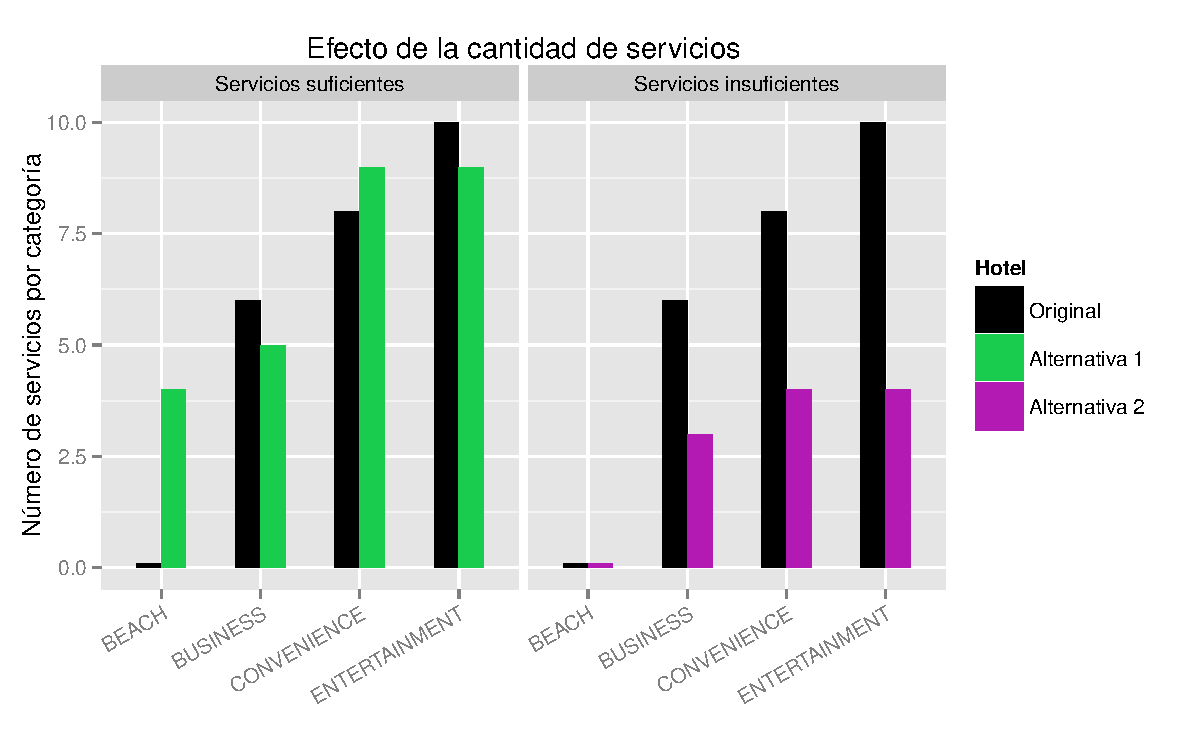
\includegraphics[width=\textwidth]{imagenes/simserv.pdf}
	\caption{\label{simserv} Ejemplos de similitud de servicios para 4 categorías distintas. El hotel verde se parece al negro porque no le faltan muchos servicios que el negro sí tiene. En contraste, al hotel morado le faltan muchos servicios.}
\end{figure}
Lo que buscaremos entonces es penalizar los servicios que le falten a un hotel a la hora de buscar candidatos. Para ello definimos la siguiente función:
\begin{defn}[Pseudodistancia \emph{hinge}]
Sean $x, y \in \mathbb{R}^n$. Definimos la pseudodistancia \emph{hinge} de $x$ a $y$ como sigue:
\[
d_h(x,y) = \sum_{k=1}^n \max\{x_k - y_k, 0\}
\]
\end{defn}
Esta función de pérdida no cumple la propiedad (\ref{dsim}) porque no es simétrica, como es evidente en la figura (\ref{fig:hingeloss}). Por lo tanto, se trata de una \emph{pseudodistancia}. Esta propiedad de $d_h(\cdot, \cdot)$ es algo positivo porque refleja justamente la asimetría de la relación entre los servicios del hotel buscado y los recomendados.
\shorthandoff{<>}
\begin{figure}
	\centering
	\begin{tikzpicture}[xscale=3.5, yscale = 3.5]
		\draw[->] (-1.2,0) -- (1.2,0);
		\draw[->] (0,-0.5) -- (0,1.2);
		\node at (1,-0.1) {$x - y$};
		\node at (-0.8,0.1) {$\max\{x - y, 0\}$};
		\node at (-0.6,1) {$|x - y|$};
		\draw[ultra thick, domain=-1:1] plot (\x, {max(\x,0)});
		\draw[red, dashed, ultra thick, domain=-1:1] plot (\x, {abs(\x)});
	\end{tikzpicture}
	\caption{Ejemplo univariado. Distancia entre $x$ y $y$ usando valor absoluto (- - -) y pérdida \emph{hinge} (---). La pérdida \emph{hinge} no penaliza el caso en que $y > x$. \label{fig:hingeloss}}
\end{figure}
\shorthandon{<>}
Aplicando esta pseudodistancia a los vectores característicos de dos hoteles $c_i$ y $c_j$ obtenemos
\[
d_h(c_i, c_j) = \sum_{k=1}^{n_c} \max\{c_{ki} - c_{kj}, 0\}
\]
La lógica detrás de esta cantidad es la siguiente: la resta $c_{ki} - c_{kj}$ representa la diferencia en número de servicios que el hotel $i$ tiene sobre el $j$ en la categoría $k$. Dado nuestro supuesto de que los servicios son perfectamente intercambiables, tenemos que $c_{ki} \geq c_{kj}$ si y sólo si el hotel $i$ es ``mejor'' en la categoría k, y por lo tanto $j$ incurrirá en una penalización de ese número por su falta de servicios. En el caso en que sea peor, es decir, cuando $c_{ki} \leq c_{kj}$, no se penaliza a $j$ y el máximo hace que se sume 0 a la distancia. En conclusión, $d_h(c_i, c_j) =$ cantidad de servicios que $j$ no tiene pero $i$ sí, tomando en cuenta los servicios en cada categoría como sustitutos perfectos.

Para etapas posteriores, cabe mencionar que dado que el número de servicios y de categorías es finito, hay una cota máxima a la distancia \emph{hinge} entre dos hoteles, digamos $M_h$, que además coincide con el número total de servicios $n_s$ (el caso se da cuando un hotel no tiene servicios y el otro tiene todos los servicios disponibles). Si bien $d_h(\cdot, \cdot)$ tiene una interpretación muy conveniente, cambiarla de escala es más útil para el modelo y hace que sea casi inmediato ver si una distancia es grande o chica, independientemente de la cantidad de servicios en el sistema. Para ello simplemente la dividimos entre $M_h$, de modo que queda entre 0 y 1, lo que también permite definir una similitud asociada:
\begin{defn}[Pseudodistancia \emph{hinge} normalizada y similitud de servicios]
Sean $x, y \in \mathbb{R}^n$. Definimos la pseudodistancia \emph{hinge} normalizada de $x$ a $y$ como sigue:
\[
d_{hn}(x,y) = \frac{1}{n_s}d_h(x,y)
\]
Definimos la similitud de servicios (o basada en \emph{hinge}) entre $x$ e $y$ como sigue:
\[
sim_h(x,y) = 1 - d_{hn}(x,y)
\]
\end{defn}

\subsection*{Similitud de perfil}

Si bien la pseudodistancia \emph{hinge} captura muy bien la falta de servicios de los hoteles candidatos, no es capaz de diferenciar adecuadamente los perfiles de los hoteles. En la gráfica (\ref{simperf}) ilustramos este hecho con dos ejemplos.
\begin{figure}[ht]
	\centering
	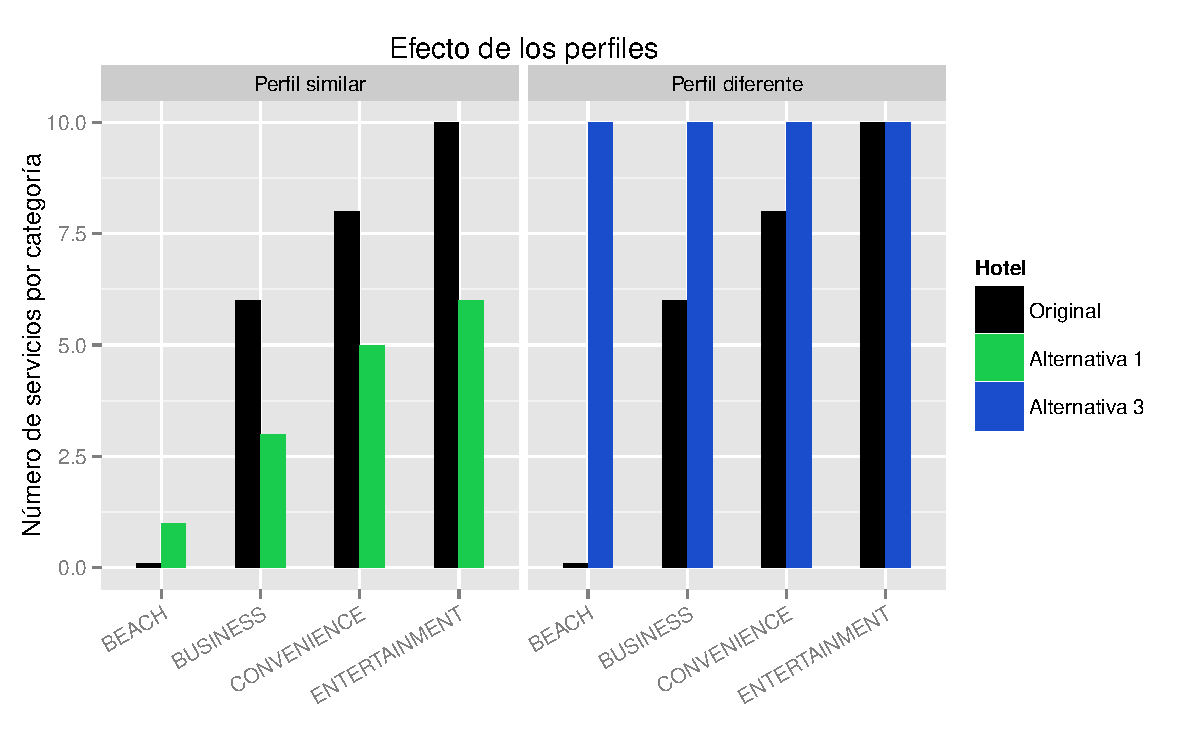
\includegraphics[width=\textwidth]{imagenes/simperf.pdf}
	\caption{\label{simperf} Ejemplos de similitud de perfil para 4 categorías distintas. El hotel verde se parece al negro porque aunque le faltan servicios, tiene aproximadamente la misma proporción de sus servicios en cada categoría. El hotel azul tiene muchos servicios, pero tiene un enfoque distinto (en este caso es un hotel de súper lujo muy enfocado a playa, mientras que el negro no tiene playa).}
\end{figure}
Una manera de modelar el perfil de un hotel es interpretando el número de servicios en cada categoría no como un número absoluto, sino como una \emph{proporción} de los servicios disponibles. Es decir, tener $m$ servicios en la categoría $k$ es mucho o poco dependiendo del número total de servicios que tiene el hotel. Como en este caso cualquier diferencia de perfil afecta, necesitamos una distancia simétrica, que definimos a continuación.
\begin{defn}[Divergencia y similitud de perfil]
Sean $x, y \in \mathbb{R}$. Defnimos la divergencia entre $x$ e $y$ como sigue:
\[
d_{div}(x, y) = \frac{1}{2}\sum_{k=1}^n \left|\frac{x_i}{\sum_j x_j} - \frac{y_i}{\sum_j y_j}\right|,
\]
es decir, la distancia absoluta entre los vectores normalizados por su suma. Definimos también la similitud de perfil (o basada en la divergencia) como
\[
sim_{div}(x,y) = 1 - d_{div}(x,y)
\]
\end{defn}
Como $d_{div}(\cdot, \cdot)$ siempre está entre 0 y 1, 
La ventaja de esta distancia (se deja como ejercicio al lector probar que en efecto cumple todas las propiedades) es que primero quita la escala y luego compara los vectores en un espacio equitativo. Cabe mencionar que bajo este criterio, el hotel verde de la gráfica (\ref{simperf}) es prácticamente idéntico al negro, incluso a pesar de que es un hotel de mucho menor categoría. El punto es que gastan sus recursos de manera similar.

Dado que los vectores normalizados suman 1 y los estamos restando, es fácil ver que por el factor de $1/2$ que incluimos en la definición, la divergencia nunca puede pasar de 1 y por lo tanto la similitud que definimos en efecto tiene sentido.

\subsection*{Similitud completa}

En las secciones anteriores resolvimos parcialmente los tres puntos críticos. Los criterios de similitud de servicios y de perfil se basan en el agrupamiento de los servicios para capturar parte de las similitudes entre los hoteles. Sin embargo, como explicamos en cada sección, ambas tienen fallas. La idea es entonces integrar las dos medidas en un criterio que sí tome en cuenta todo. El problema es cómo hacerlo sin perder información y dándole un peso apropiado a cada una.

De este punto en adelante trabajaremos nuevamente con similitudes, porque son más cómodas para razonar y porque además son equivalentes a sus distancias asociadas. Dado que tanto la similitud de servicios como la de perfil están en escalas equiparables, una manera razonable de combinarlas es promediándolas. Sin embargo, podrían tener diferentes niveles de variabilidad, por lo que es prudente permitir la posibilidad de utilizar una ponderación distinta de $1/2$.
\begin{defn}[Similitud entre hoteles]
Sea $\alpha \in (0,1)$ y sean $i, j$ hoteles en $\mathcal{H}$. Definimos la similitud con parámetro $\alpha$ entre $i$ y $j$ como sigue:
\[
sim_\alpha(c_i, c_j) = \alpha sim_h(c_i, c_j) + (1 - \alpha) sim_{div}(c_i, c_j)
\]
\end{defn}
Cabe mencionar que como la similitud entre hoteles no es simétrica porque está basada en parte en la similitud de servicios. Es decir, no necesariamente se cumple que $sim_\alpha(c_i, c_j) = sim_\alpha(c_j, c_i)$.

Ya habiendo establecido la forma de combinar las dos medidas de similitud, el siguiente paso es elegir un valor apropiado de $\alpha$, que de preferencia sea óptima con respecto a algún criterio. Para ello, hay que notar que aunque ambas similitudes están entre 0 y 1, podrían tener niveles de variación y medias distintos, por lo que utilizar $\alpha = 1/2$ podría no ser una buena idea. Ilustramos este hecho en la figura (\ref{alpha}).
\begin{figure}[ht]
	\centering
	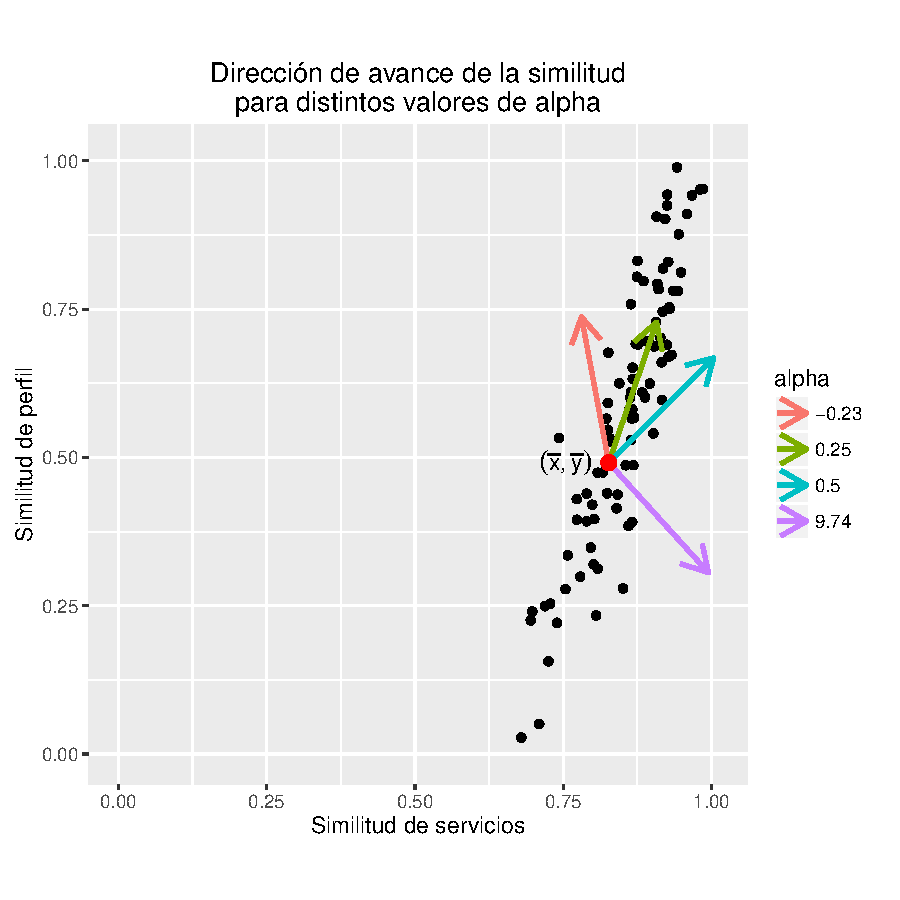
\includegraphics[width=0.7\textwidth]{imagenes/alpha.pdf}
	\caption{\label{alpha} La elección de $\alpha$ determina la dirección en la que avanza la similitud total al variar la de servicios y la de perfil.}
\end{figure}
Dado que lo que queremos es identificar hoteles similares, una buena manera de decidir el valor de $\alpha$ es utilizando la que maximice la varianza explicada por la similitud completa. En el ejemplo, $\alpha = 1/2$ probablemente sería similar a avanzar en la flecha pequeña de la derecha, pero es claro que avanzando en la dirección de la de en medio estaríamos tratando ambas similitudes de manera más equitativa. Proponemos utilizar un Análisis de Componentes principales para calcular la $\alpha$ óptima.

Con la alpha buena se llama score


\section{Distancia: filtro dinámico}
\section{Precios dinámicos}
\section{Implementación}
número de servicios
número de categorías
plan de alimentos
\section{Comentarios}
Por qué no distancia absoluta?
No es personalizado, sino de hoteles similares.
[Ver presentación para qué sí/no es o podría ser]

% ----------------------------------------------------------------------------------------------------
\chapter{Obtención de la información}
\section{Formato necesario para el modelo}
\section{Calidad de la información}
\section{Sistema de respaldo}

% ----------------------------------------------------------------------------------------------------
\chapter{Desempeño}
Casos de éxito, incluso en zonas ralas.
Red de interconexiones, incluyendo PageRank.

% ----------------------------------------------------------------------------------------------------
\chapter{Trabajo futuro}
Porcentaje dinámico en forma de `U' para el tope de precio.
















\end{document}